\chapter{Network Prototyping Router Boards}\label{sec:hardware}

\section{Objectives}\label{sec:hardware:objectives}

Hardware has been developed to provide a platform on which a prototype of the toolkit will be implemented for demonstration purposes. Given the demonstration nature, the hardware a) must be flexible enough that different networks can be prototyped b) must be simple enough that it can be easily assembled with available equipment and c) must utilize a mainstream embedded processor.

\section{Background}\label{sec:hardware:background}

The mainstream embedded processor selected for the prototype toolkit is the TMS320F2808 (a.k.a. F2808) Digital Signal Controller (DSC) from Texas Instruments (TI). The F2808 contains a C2000 Digital Signal Processing (DSP) core running at 100 MHz, 36 KB of RAM\footnote{The Minimum Addressable Data Unit (MADU) is 16 bits, not 8 bits, which makes addressing more complicated}, 128 KB of Flash memory, and a variety of peripherals. The F2808 comes in a 100 pin LQFP package, shown in Figure \ref{fig:hardware:f2808_pin_diagram}. The device is called a DSC because it has the processing core of a traditional DSP chip combined with the peripherals of a traditional microcontroller. The block diagram for the F2808 is shown in Figure \ref{fig:hardware:f2808_block_diagram}. \cite{ref:2006-ti-f2808_users_guide}. The toolkit will make use of the RAM and FLASH memory, General Purpose Input/Output (GPIO) pins, and the Serial Peripheral Interface (SPI) hardware.

\begin{figure}[ptb]
	\begin{centering}
		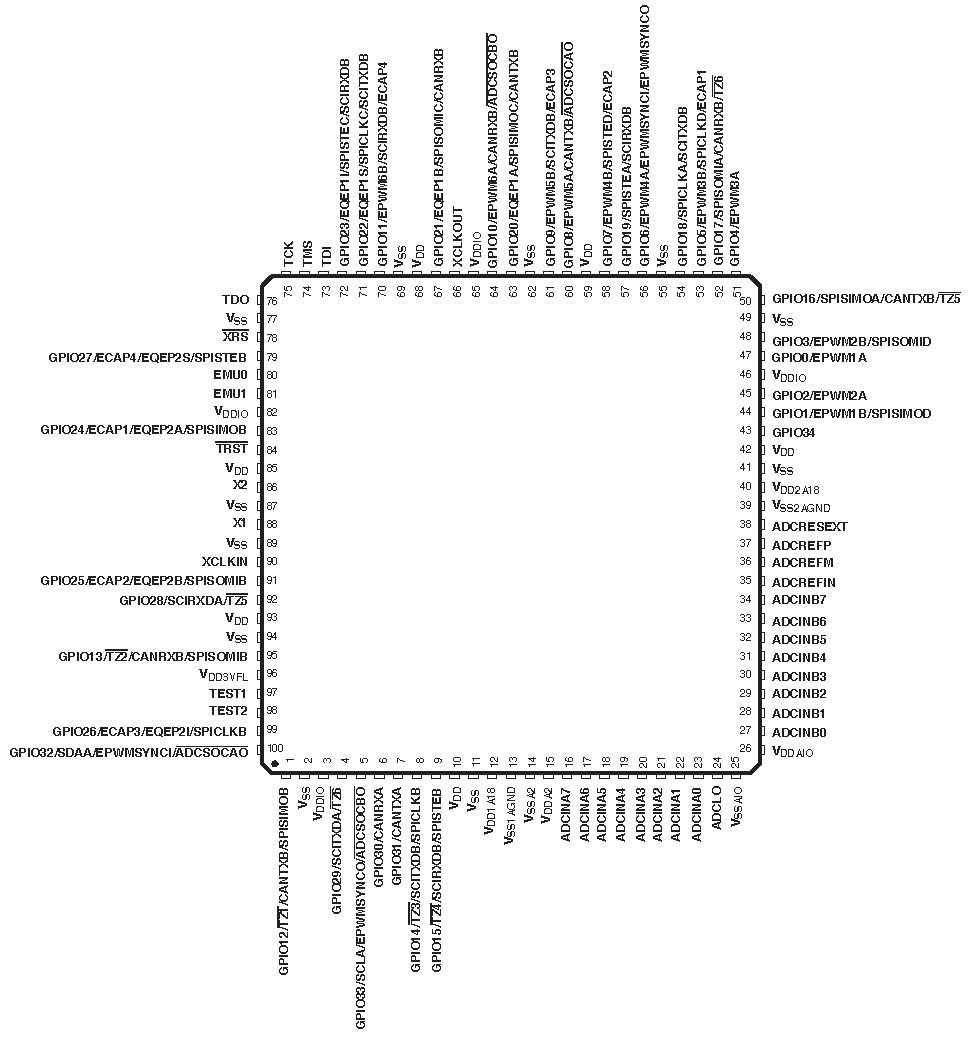
\includegraphics[scale=0.75]{Hardware/Figures/hardware-f2808_pin_diagram.pdf}
		\caption[F2808 Pin Diagram]{F2808 Pin Diagram \cite{ref:2006-ti-f2808_users_guide}}
		\label{fig:hardware:f2808_pin_diagram}
	\end{centering}
\end{figure}

\begin{figure}[ptb]
	\begin{centering}
		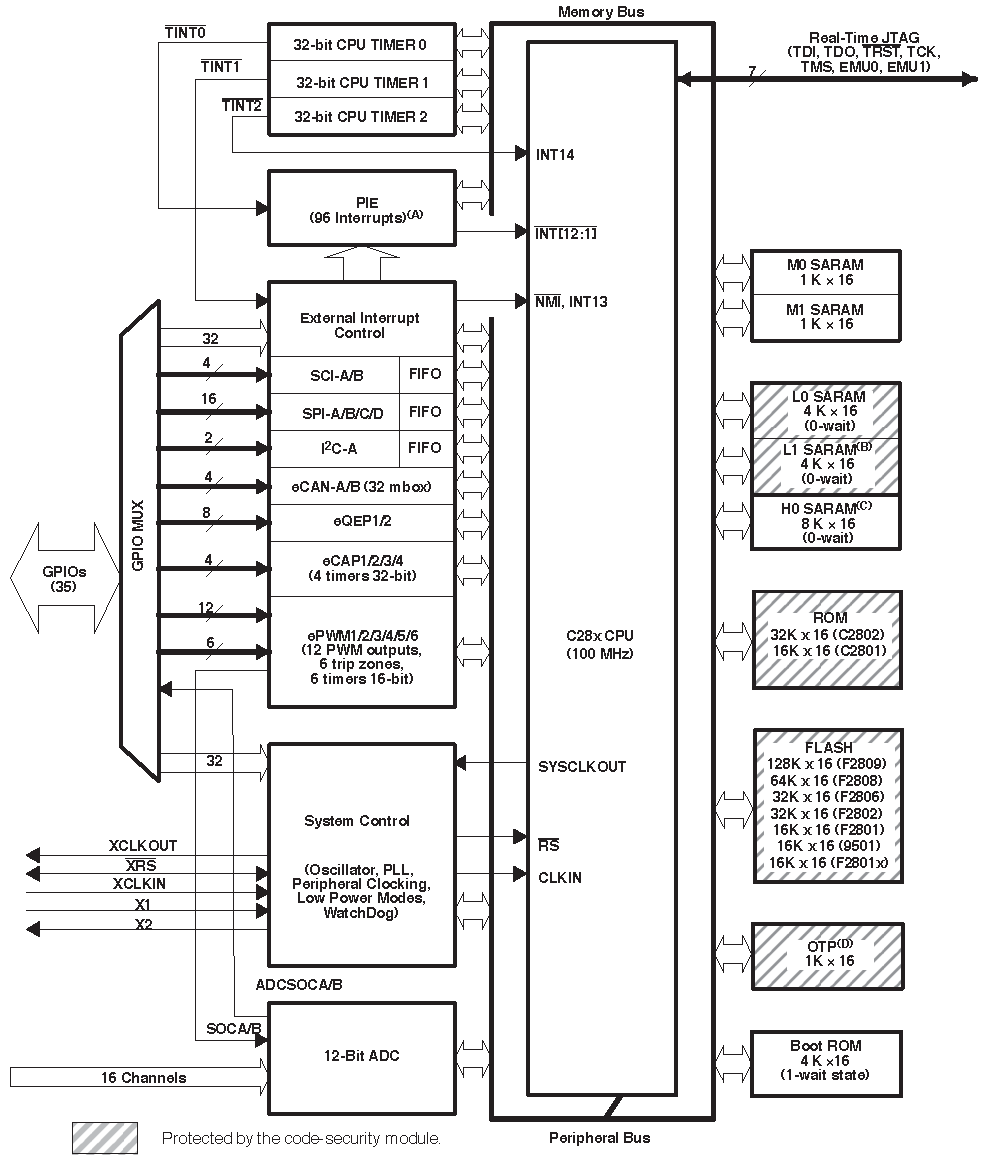
\includegraphics[scale=0.75]{Hardware/Figures/hardware-f2808_block_diagram.pdf}
		\caption[F2808 Block Diagram]{ F2808 Block Diagram \cite{ref:2006-ti-f2808_users_guide}}
		\label{fig:hardware:f2808_block_diagram}
	\end{centering}
\end{figure}

The F2808 contains one 128 KB block of flash memory, one 1 KB block of One Time Programmable memory, one 4 KB block of Boot ROM that comes pre-programmed with a simple boot loader, and three blocks of RAM totaling $\textrm{18k} \times \textrm{16b}$. The full memory map is shown in Figure \ref{fig:hardware:f2808_memory_map}, although this project only utilizes flash and RAM. The F2808's memory structure has several interesting aspects to it. One aspect that must be considered is that RAM is partitioned into five blocks: M0 and M1 SARAM, L0 and L1 SARAM, and H0 SARAM. TI's software (e.g. DSP/BIOS and the compiler) is set up to view M0 and M1 SARAM as a single block (MSARAM) and L0 and L1 SARAM as a single block (LSARAM), but keeps H0SARAM as a separate block, and the user defines where they want code and data to be stored. The F2808 has three peripheral frames that contain the registers for the peripheral on the device. Two of the frames are marked as ``protected,'' which means that their contents cannot be modified unless the assembly command "EALLOW" is issued first. The PIE vector is interrupt related. \cite{ref:2006-ti-f2808_users_guide}

\begin{figure}[ptb]
	\begin{centering}
		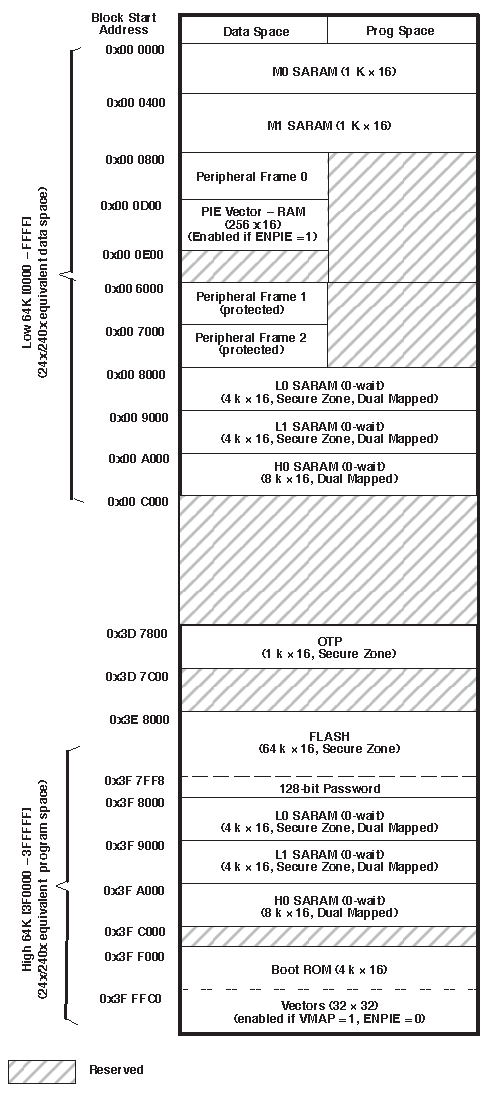
\includegraphics[scale=0.75]{Hardware/Figures/hardware-f2808_memory_map.pdf}
		\caption[F2808 Memory Map]{F2808 Memory Map \cite{ref:2006-ti-f2808_users_guide}}
		\label{fig:hardware:f2808_memory_map}
	\end{centering}
\end{figure}

The C2000 core supports 14 interrupts, INT1 through INT14, shown in Figure \ref{fig:hardware:f2808_interrupts_block_diagram}. Because this isn't enough interrupts to service all of the peripherals, TI created the Peripheral Interrupt Expansion (PIE) mechanism, which occupies INT1 through INT12. Interrupts associated with the peripherals and GPIO interrupts (XINTx) use the PIE, along with the watchdog and CPU timer 0 interrupts. INT 14 is used for CPU timer 2, and INT13 is multiplexed with timer 1 and a few other odds and ends. The PIE, shown in Figure \ref{fig:hardware:f2808_pie}, essentially multiplexes a series of related interrupts into a single CPU interrupt. When an interrupt occurs, the CPU automatically fetches the interrupt vector from the PIE and sets the appropriate interrupt flag. Interrupt Service Routines (ISRs) are automatically called based on the interrupt in the PIE. Thus, it is not necessary for the user to write an ISR to service INTx directly and then read the PIE to determine the specific interrupt. After the PIE is initially configured, peripheral interrupts act as if the PIE and core interrupts were a single unified system.\cite{ref:2006-ti-f2808_system_control_and_interrupts}

\begin{figure}[ptb]
	\begin{centering}
		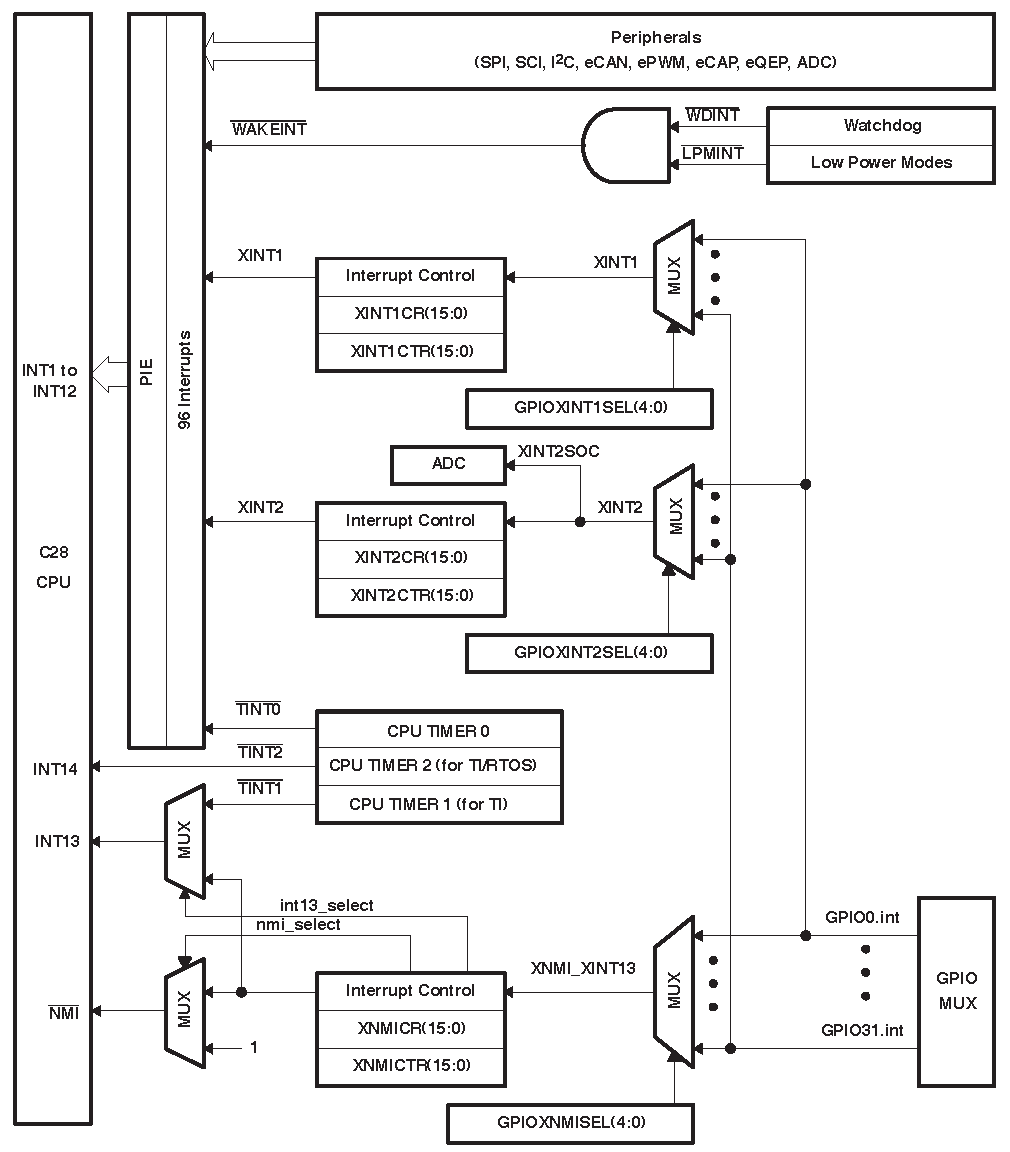
\includegraphics[scale=0.75]{Hardware/Figures/hardware-f2808_interrupts_block_diagram.pdf}
		\caption[F2808 Interrupt Block Diagram]{F2808 Interrupt Block Diagram \cite{ref:2006-ti-f2808_system_control_and_interrupts}}
		\label{fig:hardware:f2808_interrupts_block_diagram}
	\end{centering}
\end{figure}

\begin{figure}[ptb]
	\begin{centering}
		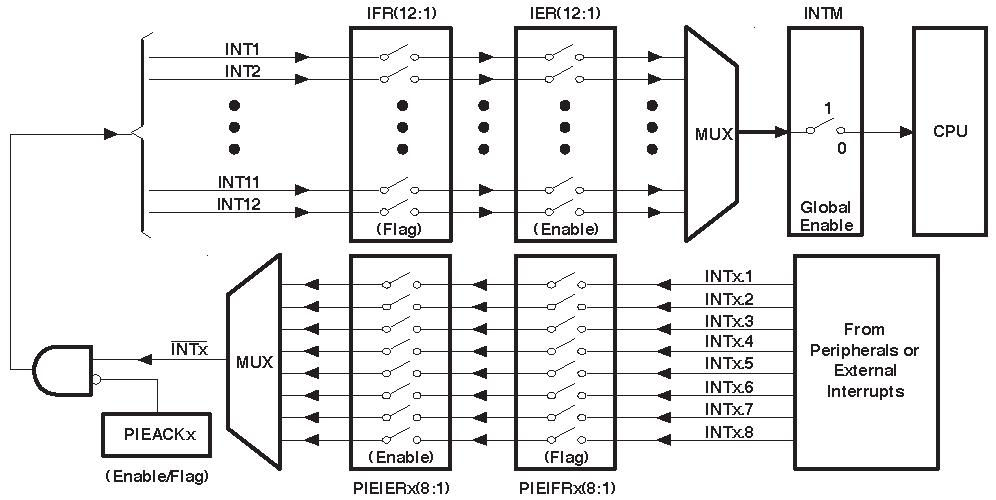
\includegraphics[scale=0.75]{Hardware/Figures/hardware-f2808_pie.pdf}
		\caption[F2808 PIE Block Diagram]{F2808 PIE Block Diagram\cite{ref:2006-ti-f2808_system_control_and_interrupts}}
		\label{fig:hardware:f2808_pie}
	\end{centering}
\end{figure}

The F2808 has thirty-five GPIO pins that are multiplexed with up to three other peripherals. Each input has a pull-up resistor that can be enabled in software. The block diagram for the GPIO system is shown in Figure \ref{fig:hardware:f2808_gpio}. The F2808 has three input qualification modes that can be selected: asynchronous, synchronous, and windowed. Asynchronous mode bypasses the input qualification stage and can only be used by peripherals that support it (such as SPI in slave mode). Synchronous mode synchronizes the input with the system clock. Windowed mode requires the input to be held for a certain number of clock cycles before the input is allowed to change. Pins can be configured as either input or output. Registers are available that allow a pin to be read (GPxDAT), set (GPxSET), cleared (GPxCLEAR), and toggled (GPxTOGGLE).

\begin{figure}[ptb]
	\begin{centering}
		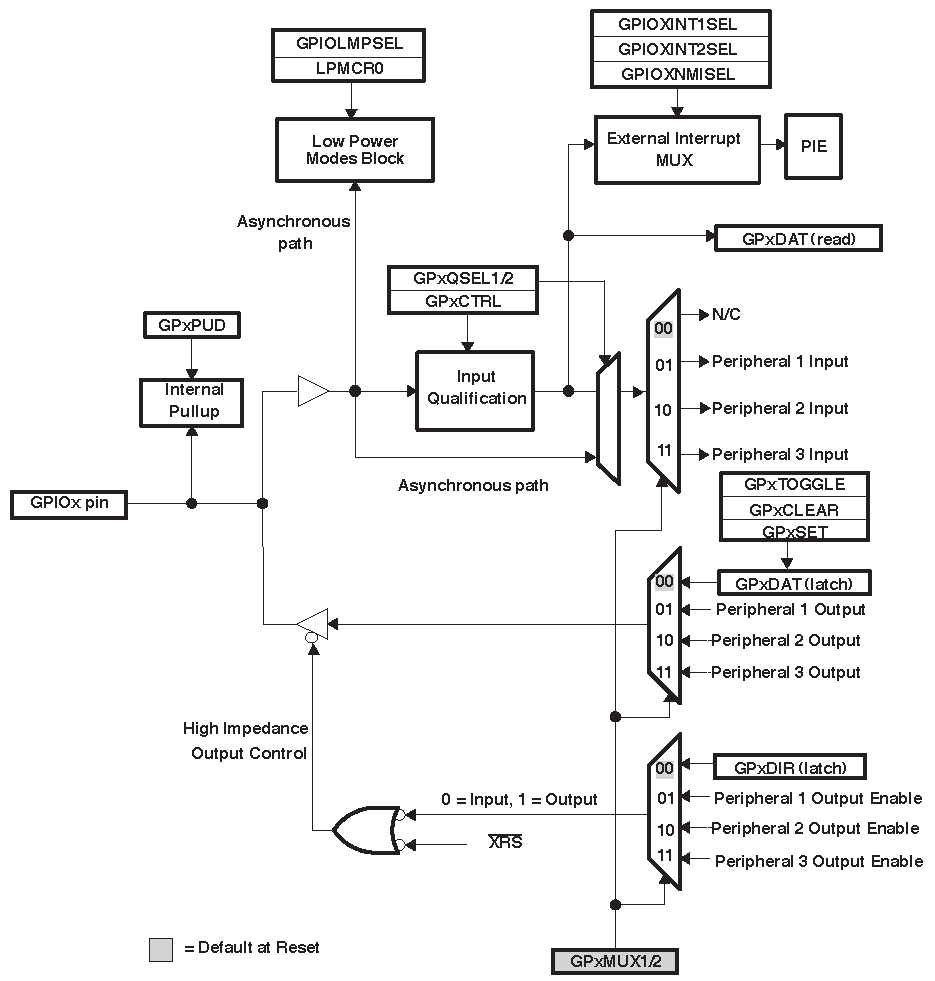
\includegraphics[scale=0.75]{Hardware/Figures/hardware-f2808_gpio.pdf}
		\caption[F2808 GPIO Block Diagram]{F2808 GPIO Block Diagram\cite{ref:2006-ti-f2808_system_control_and_interrupts}}
		\label{fig:hardware:f2808_gpio}
	\end{centering}
\end{figure}

The F2808 contains four SPI ports, and the block diagram for one port is shown in Figure \ref{fig:hardware:f2808_spi}. The F2808 uses a single buffer for both transmitting and receiving because transmission and receiving are closely linked in the SPI. As data is shifted out to be transmitted, new data is shifted in as it is received. The F2808 allows characters to range from 1 bit long to 16 bits long. The clock can be configured to run from 56 kbps up to 25 Mbps when the device's clock speed is 100 MHz. The F2808 has optional 16 word FIFO buffers for both receive and transmit. When using the FIFOs, three receive interrupt sources and one transmit interrupt source are available to the developer. A receive interrupt can be caused when the receive buffer contains  words, the receive buffer has overflowed, or an internal error is detected. \cite{ref:2006-ti-f2808_spi} The theory and operation of the SPI is described in more detail in Chapter \ref{sec:spi}. 

\begin{figure}[ptb]
	\begin{centering}
		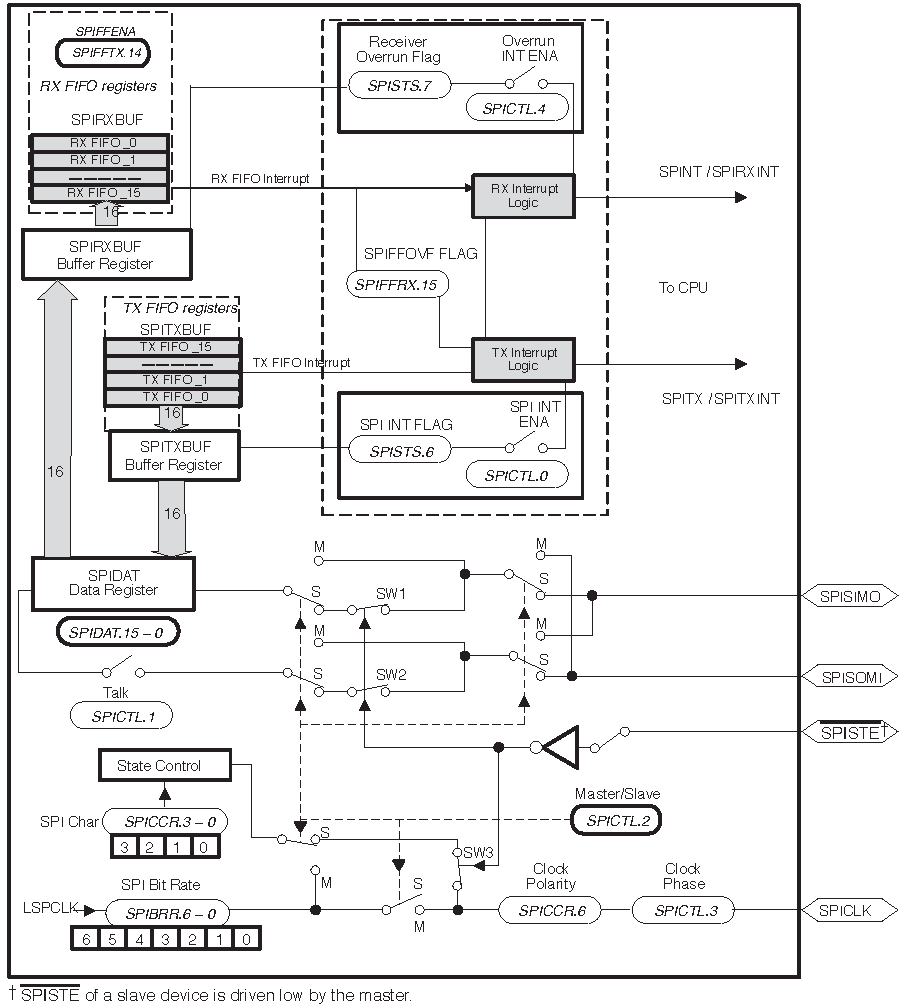
\includegraphics[scale=0.75]{Hardware/Figures/hardware-f2808_spi.pdf}
		\caption[F2808 SPI Block Diagram]{F2808 SPI Block Diagram\cite{ref:2006-ti-f2808_spi}}
		\label{fig:hardware:f2808_spi}
	\end{centering}
\end{figure}

\section{Methodology}\label{sec:hardware:methodology}

Circuit boards have been designed containing a single F2808 that can be easily interconnected using ribbon cables. This configuration allows easy prototyping of a variety of network configurations, satisfying the first objective. The complexity of the power and debug circuitry necessary to support multiple processors is unnecessary on a single-processor board, thus simplifying the design greatly. In addition, all surface mount components in the design have external pins that can be soldered using a standard soldering iron. This design simplicity and component selection satisfies the second objective. Given the clock speed, memory, and peripheral specifications of the F2808, the third objective is also met. Each board is self-contained, only requiring a DC input from an unregulated AC to DC transformer in the range of 4.5 V to 7 V and ribbon cables to connect to other boards, which reduces the complexity of auxiliary circuitry.
Each board provides several peripherals, shown in Figure \ref{fig:hardware:block_diagram}. Each board provides its own power protection and regulation circuitry. The Joint Test Action Group (JTAG) connector is used to program and debug the firmware on the boards. The seven segment display is used to indicate the assigned address of the node and the current state of the firmware. The DIP switches are used to set runtime parameters of the firmware.

\begin{figure}[ptb]
	\begin{centering}
		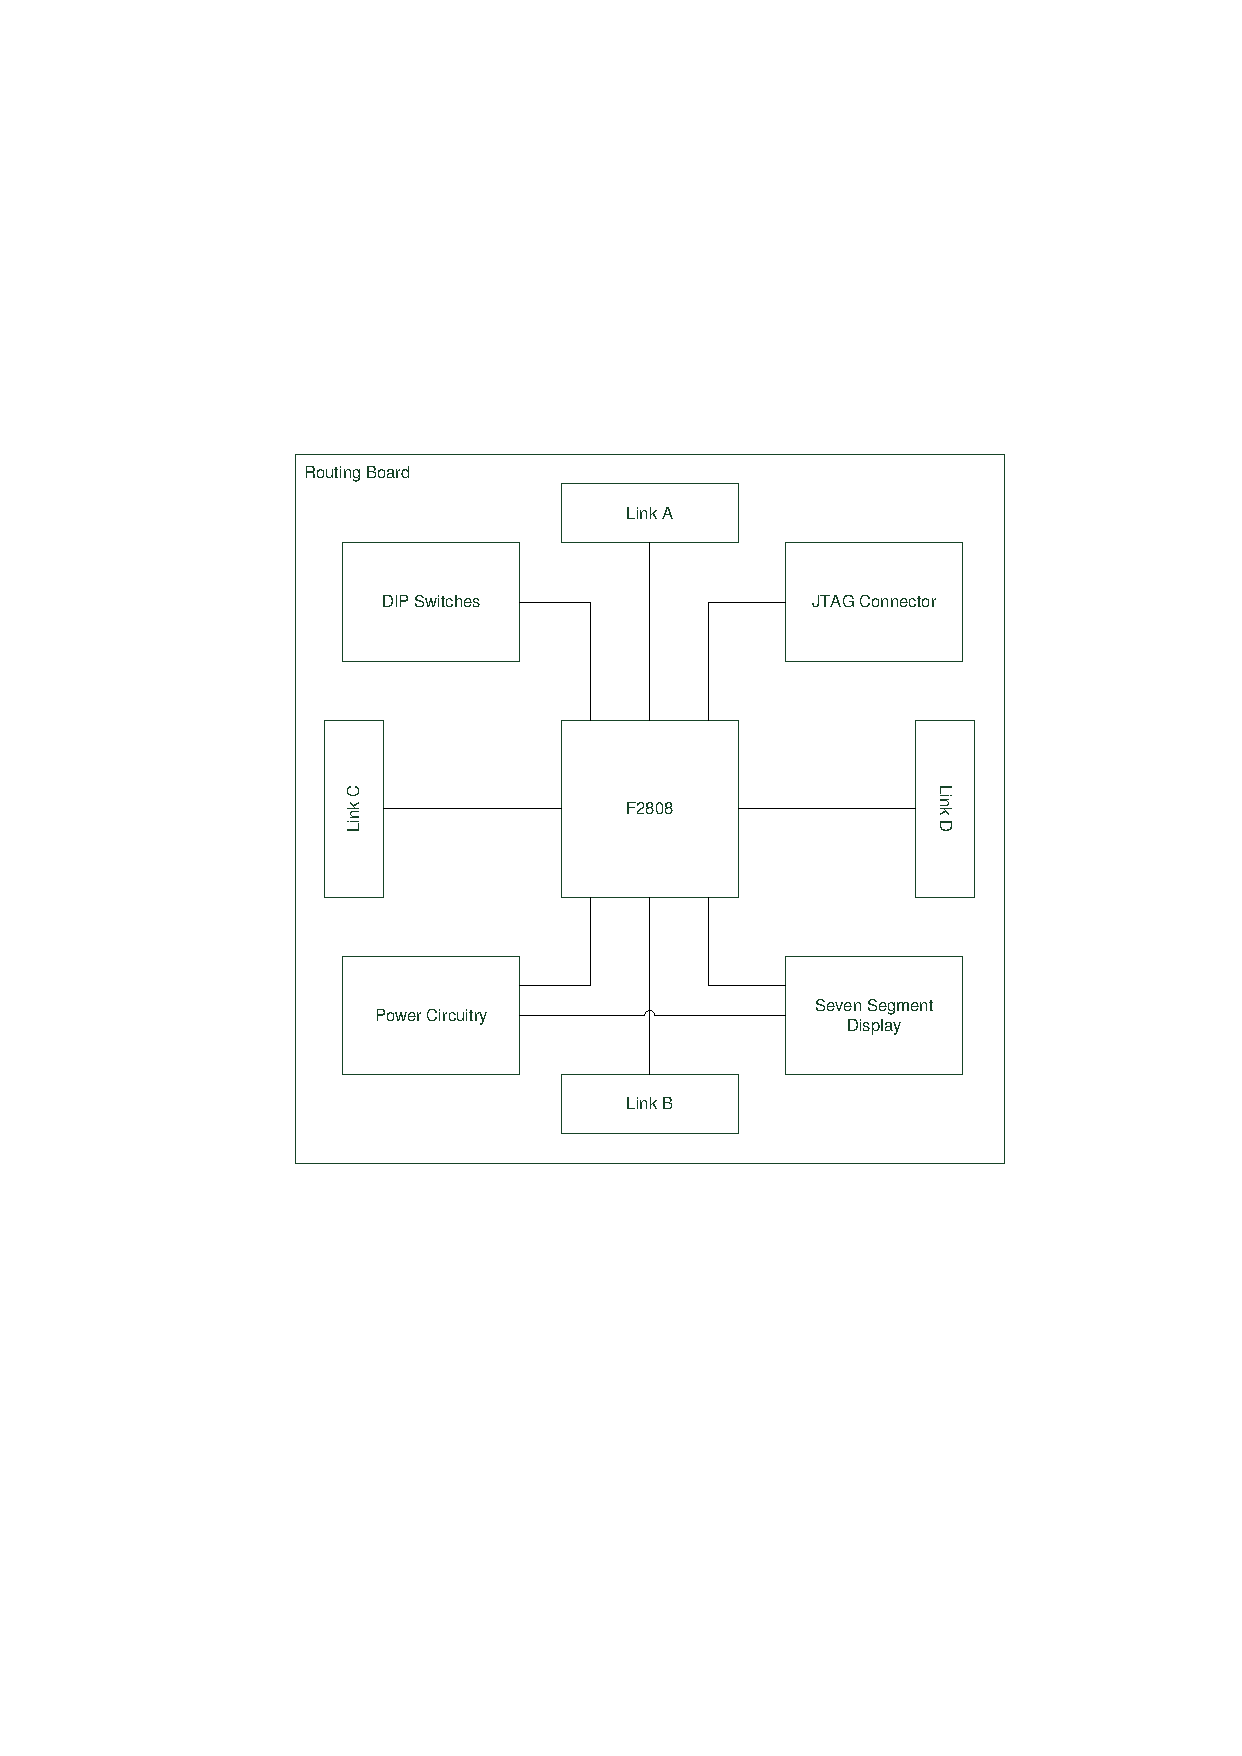
\includegraphics[width=4in]{Hardware/Figures/hardware-block_diagram.pdf}
		\caption{Prototyping Board Block Diagram}
		\label{fig:hardware:block_diagram}
	\end{centering}
\end{figure}

\section{Implementation}\label{sec:hardware:implementation}

The boards are implemented on a four layer printed circuit board that was manufactured by Sierra Circuits, Inc. The schematic for the board is shown in Figure \ref{fig:hardware:schematic}, and the layout is shown in Figure \ref{fig:hardware:layout}. Expanded views of the layout are shown in Appendix \ref{sec:appendix:expanded_layout}.

\begin{landscape}
	\begin{figure}[ptb]
		\begin{centering}
			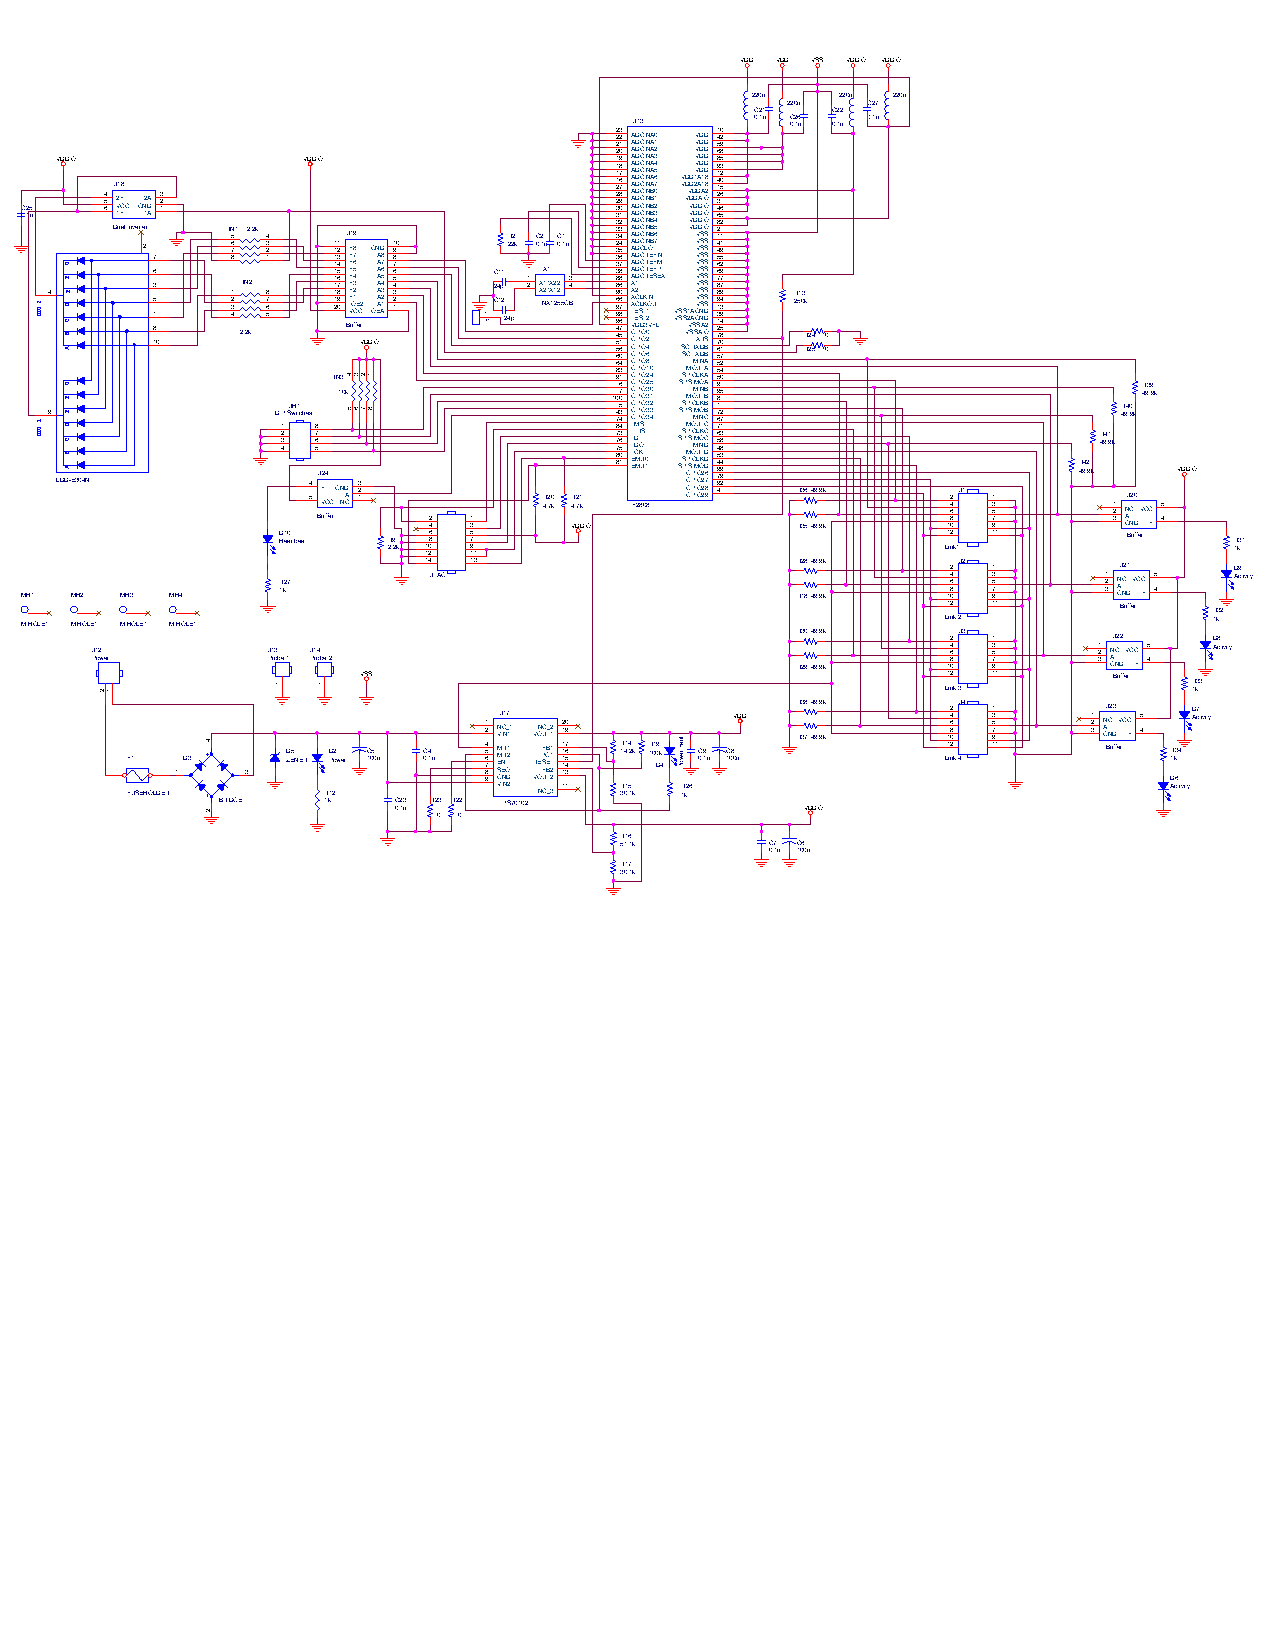
\includegraphics[width=8.25in]{Hardware/Figures/hardware-schematic.pdf}
			\caption{Prototyping Board Schematic}
			\label{fig:hardware:schematic}
		\end{centering}
	\end{figure}
\end{landscape}

\begin{figure}[ptb]
	\begin{centering}
		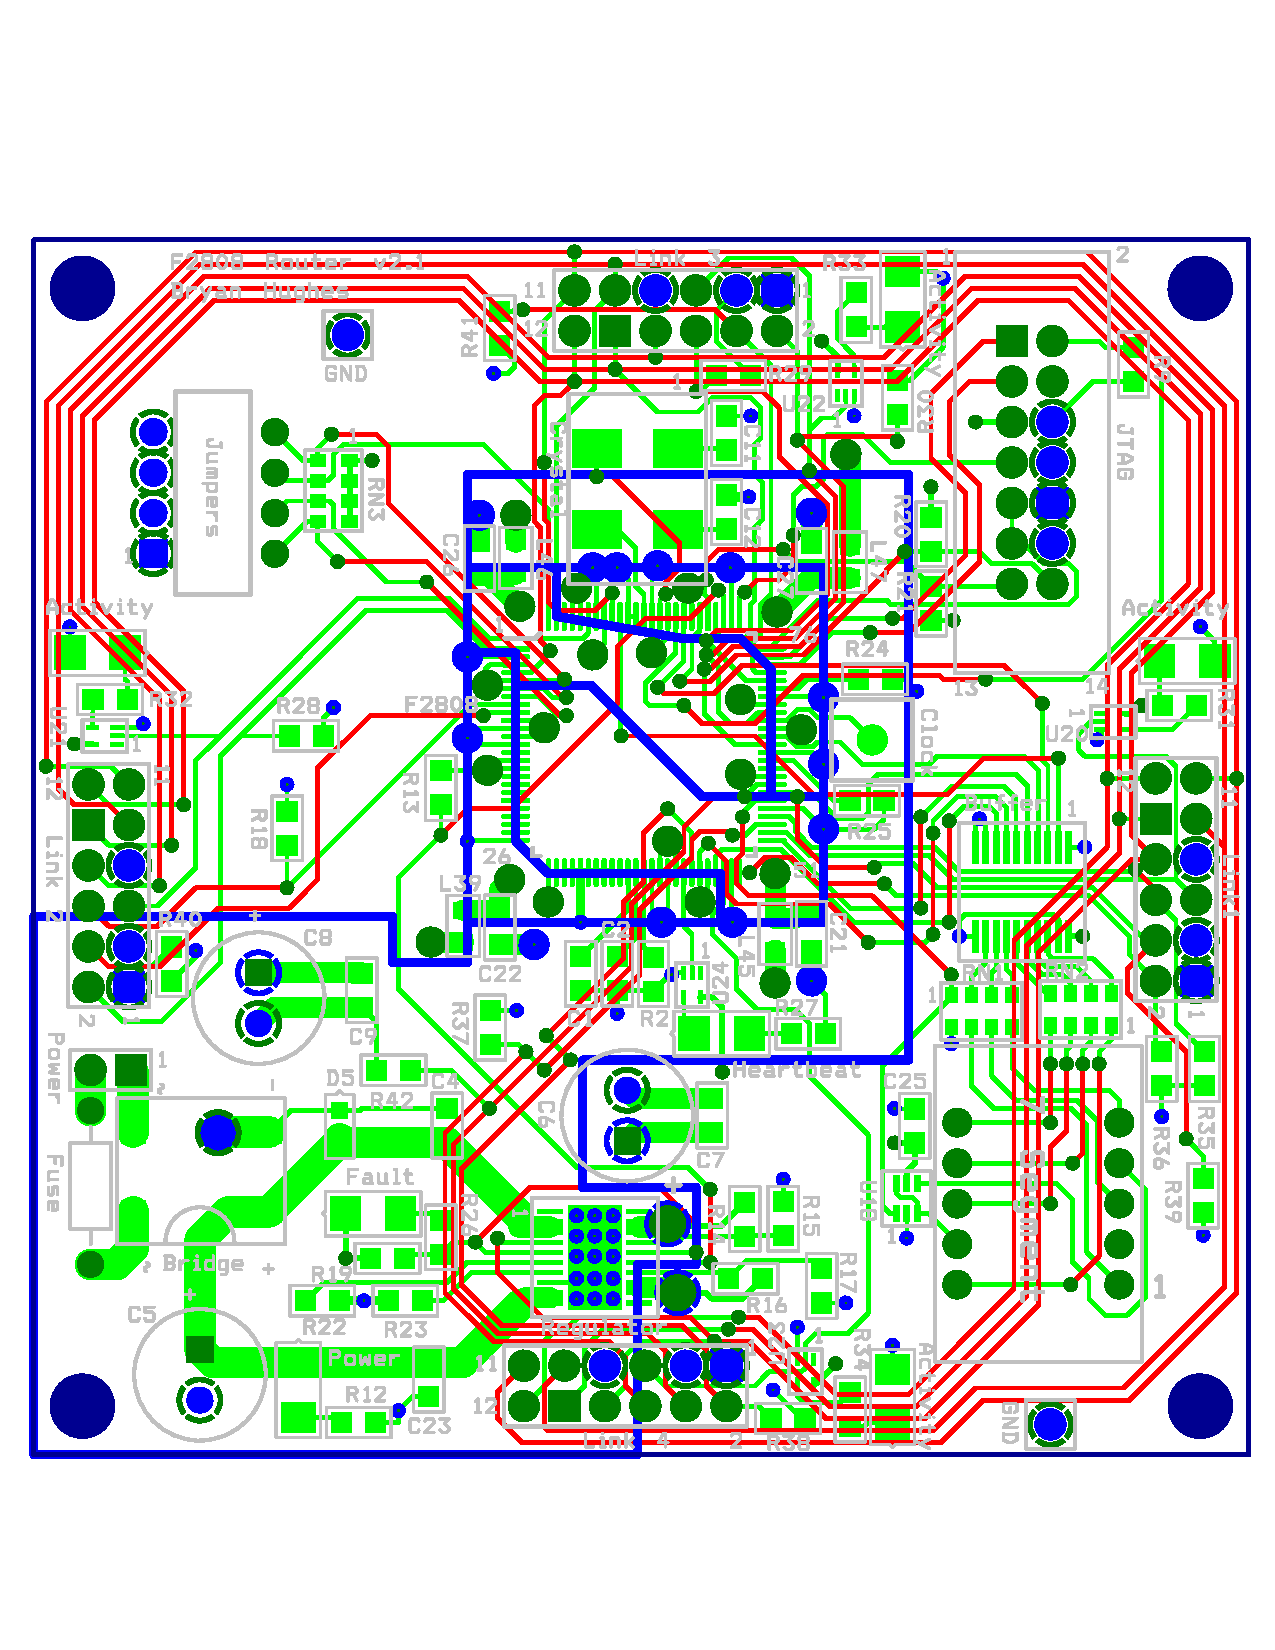
\includegraphics[width=6in]{Hardware/Figures/hardware-layout.pdf}
		\caption{Prototyping Board Layout}
		\label{fig:hardware:layout}
	\end{centering}
\end{figure}

The power delivery circuit is divided into power protection circuitry and power regulation circuitry. The power protection circuitry is shown in Figure \ref{fig:hardware:schematic_power_protection}. A diode bridge is included to prevent the polarity of the input power from being swapped. A fuse is added to prevent amperage overages from damaging the device, such as from heavy power irregularities in the AC supply (e.g. lightning). Since fuses are slow to respond, a Zener diode is included to prevent rapid changes in voltage over 6 Volts from damaging the device. Power regulation, shown in Figure \ref{fig:hardware:schematic_power_regulation}, is accomplished using the TPS70102 low dropout linear regulator from TI. The TPS70102 is designed specifically for use with TI's DSPs, which require 1.8 V for the processing core and 3.3 V for the I/O. The F2808 has very specific requirements on power-up timing: the 1.8 V supply must be at 80\% of its max voltage before the 3.3 V line can begin to rise above 0 V, and the reset line must be asserted for at least 10 ms. The TPS70102 handles all of the sequencing, which greatly simplifies the design. The TPS70102 is an adjustable device, so the resistors in the circuit are used to specify 1.8 V and 3.3 V operation, with the 1.8 V supply being sequenced first. Power and Power Fault LEDs were added for improved user feedback. 0.1 \textmu F and 100 \textmu F capacitors are used to filter the power.\cite{ref:2007-ti-tps70102}

\begin{figure}[ptb]
	\begin{centering}
		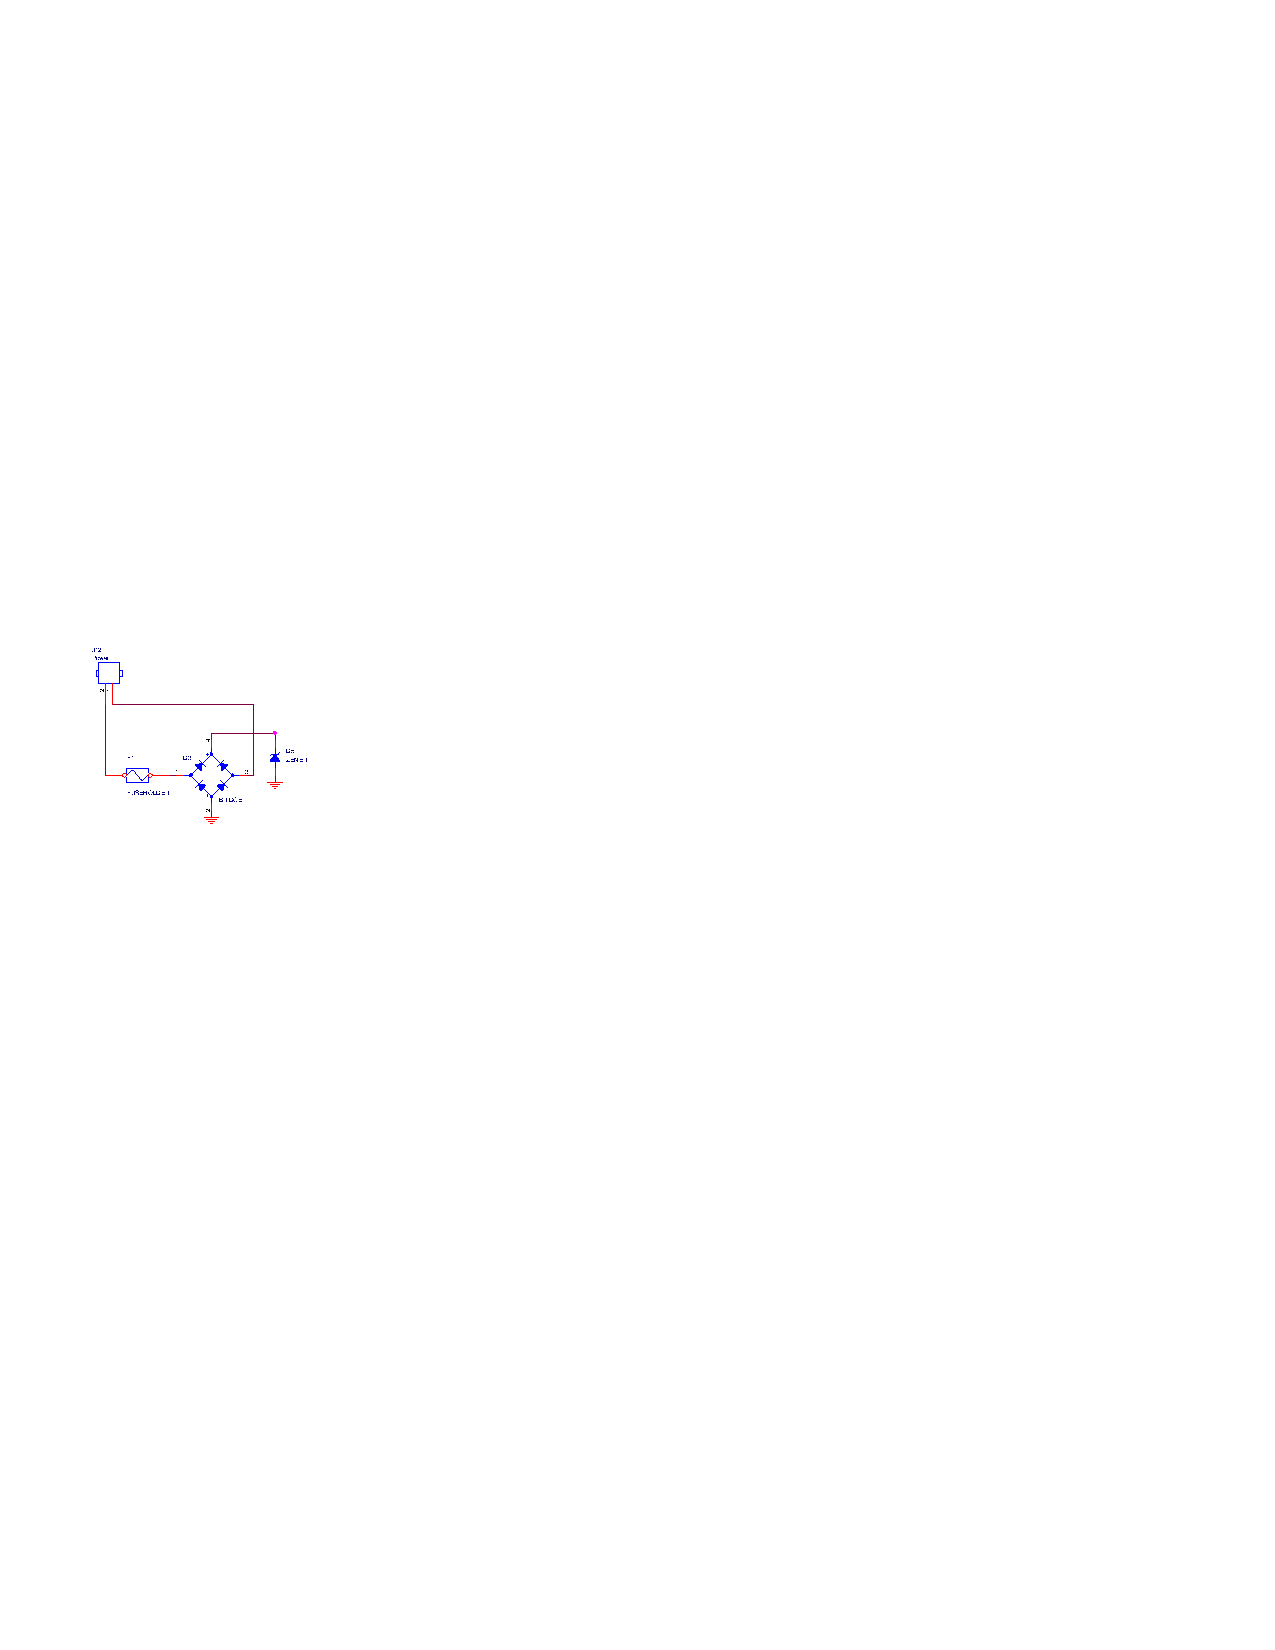
\includegraphics[scale=1.3]{Hardware/Figures/hardware-schematic_power_protection.pdf}
		\caption{Prototyping Board Power Protection Circuitry}
		\label{fig:hardware:schematic_power_protection}
	\end{centering}
\end{figure}

\begin{figure}[ptb]
	\begin{centering}
		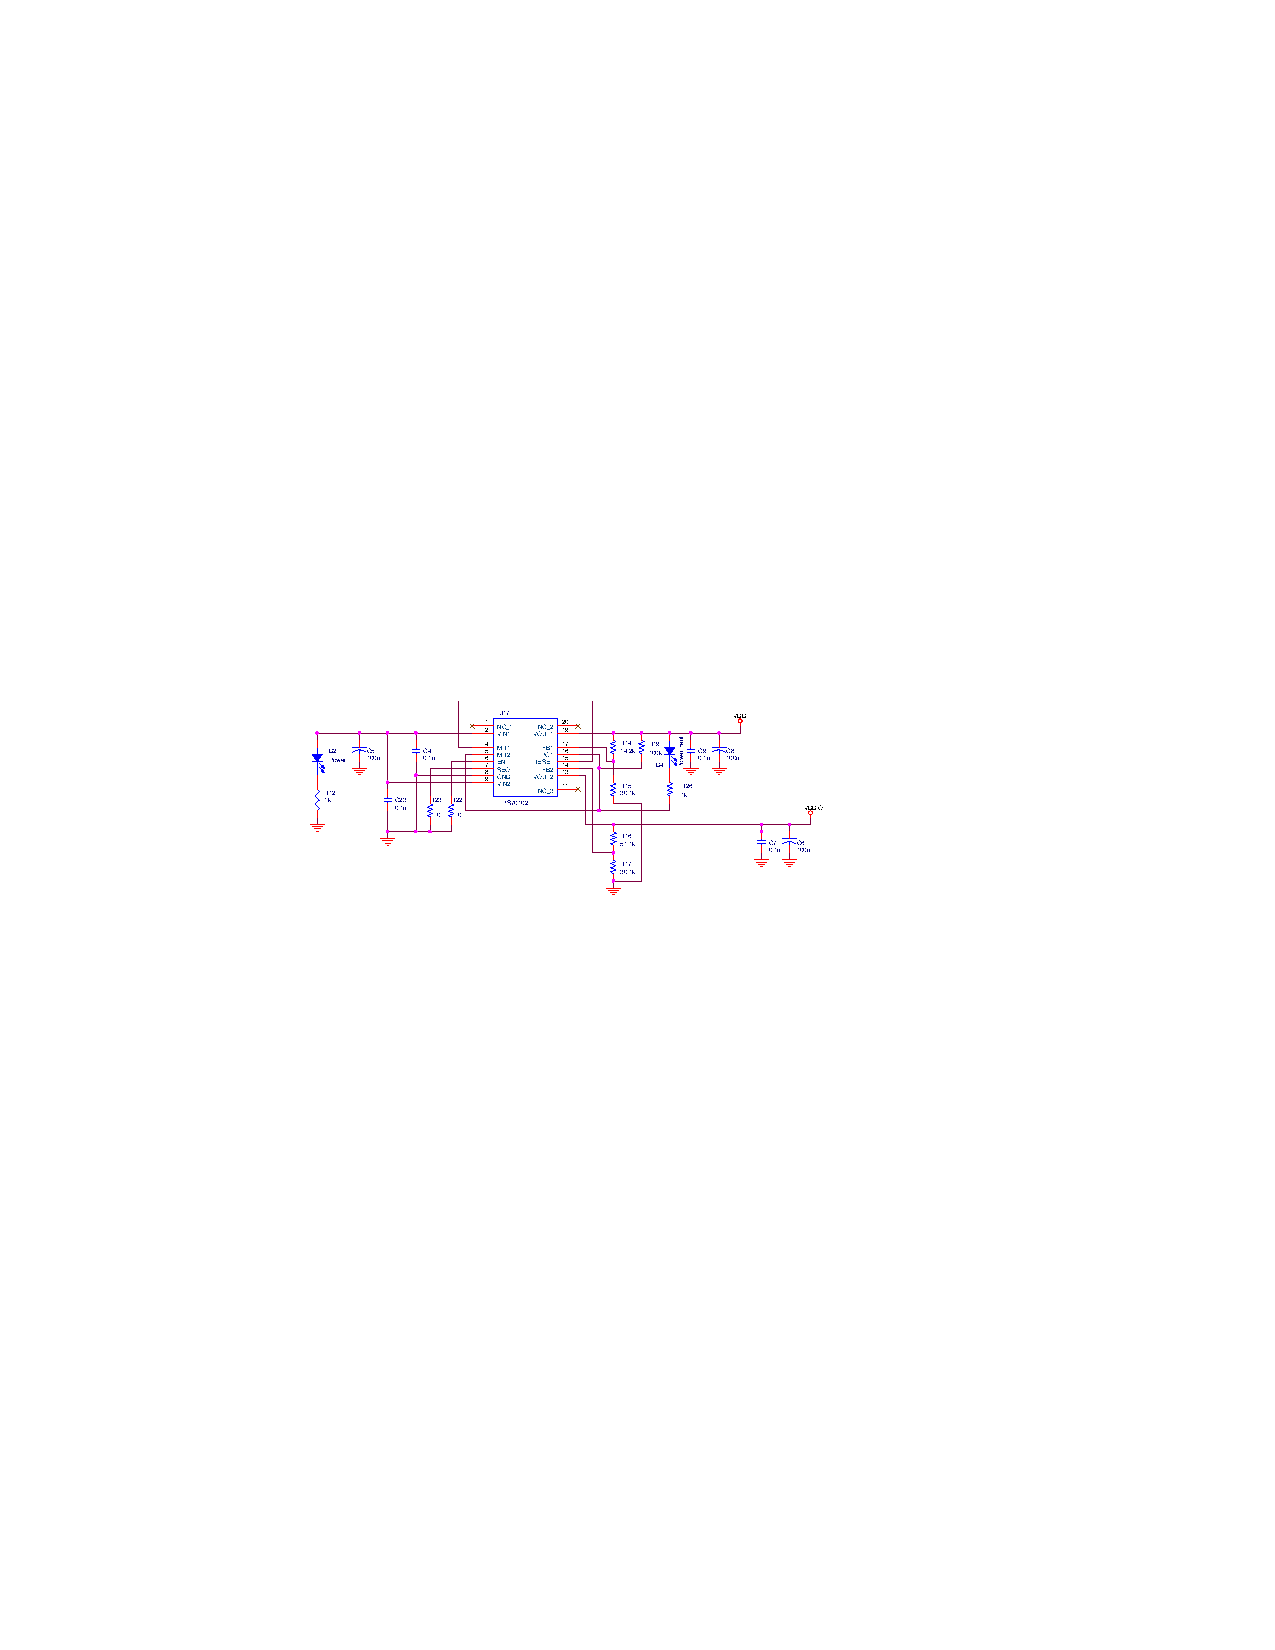
\includegraphics[scale=1.3]{Hardware/Figures/hardware-schematic_power_regulation.pdf}
		\caption{Prototyping Board Power Regulation Circuitry}
		\label{fig:hardware:schematic_power_regulation}
	\end{centering}
\end{figure}

The F2808 is connected to the power via a series of chokes and bypass capacitors in order to further smooth out the power. A heartbeat LED is connected via a discrete buffer that periodically flashes to indicate that the firmware is running. A 20 MHz crystal is connected to drive the clock. The JTAG and reset lines are implemented according to the data sheet. Four DIP switches in a single package are connected to the F2808 with a 10 k\textohm pull-up resistor array. These connections are shown in \ref{fig:hardware:schematic_core}.

\begin{figure}[ptb]
	\begin{centering}
		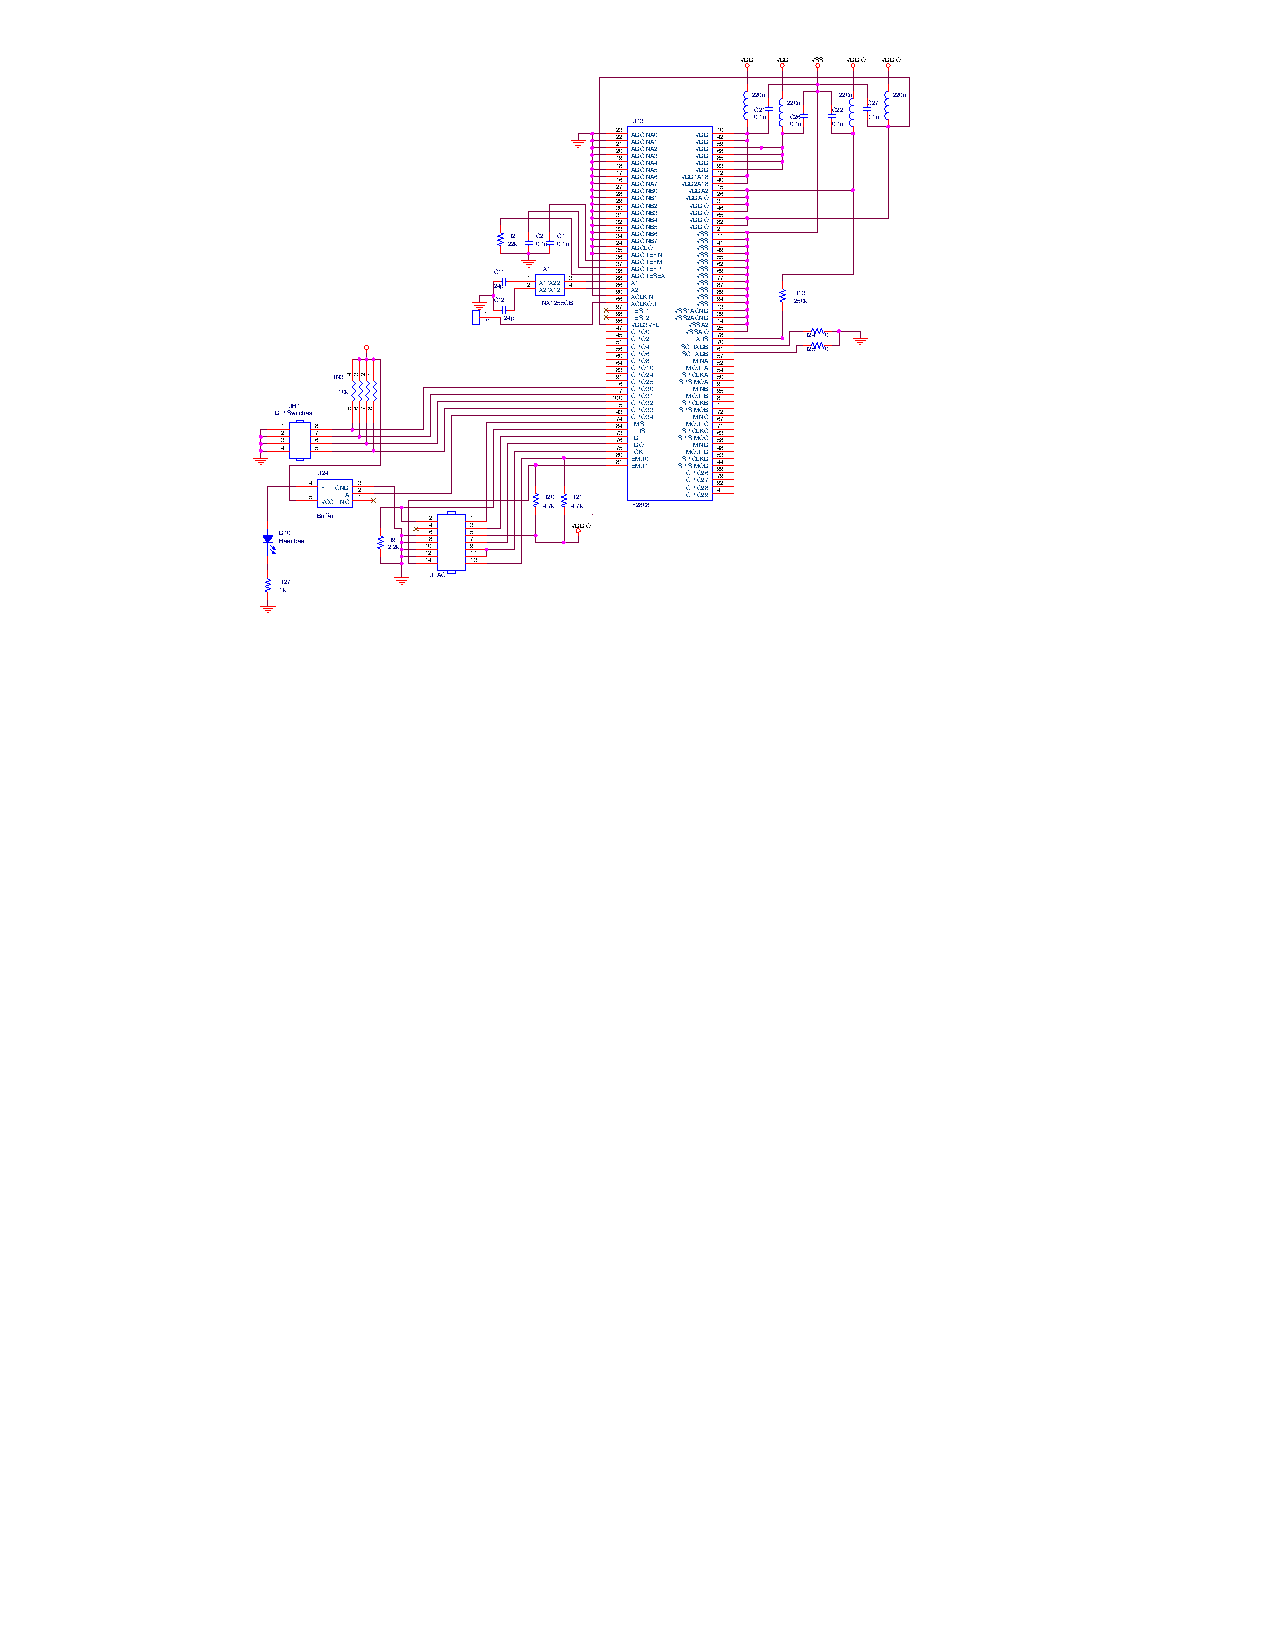
\includegraphics[scale=1.3]{Hardware/Figures/hardware-schematic_core.pdf}
		\caption{Prototyping Board Core Circuitry}
		\label{fig:hardware:schematic_core}
	\end{centering}
\end{figure}

The seven segment display requires a bit more support circuitry in order to make it work. The seven segment display operates by only lighting one digit at a time, and switching between them fast enough that the human eye perceives both digits as being lit continually. This procedure reduces the number of pins necessary to operate the device. The seven segment display is implemented as an LED array with each digit sharing a common cathode. To light a digit, the common cathode is driven low, and the segments to light are driven high. Driving the common cathode high turns off that digit. Because one digit will always be high, and the other always low, a dual inverter gate is used to drive both digits using a single logic pin on the F2808. The first gate is used as a buffer because the F2808 can't sink or source enough current to drive the cathode directly. The input on the second gate is connected to the output of the first gate, and the output of the second gate is connected to the common cathode on the second digit. This configuration ensures that when one digit is on, the other is off. An octal buffer is used to drive the individual anodes high. This mechanism is shown in Figure \ref{fig:hardware:schematic_seven_segment}.

\begin{figure}[ptb]
	\begin{centering}
		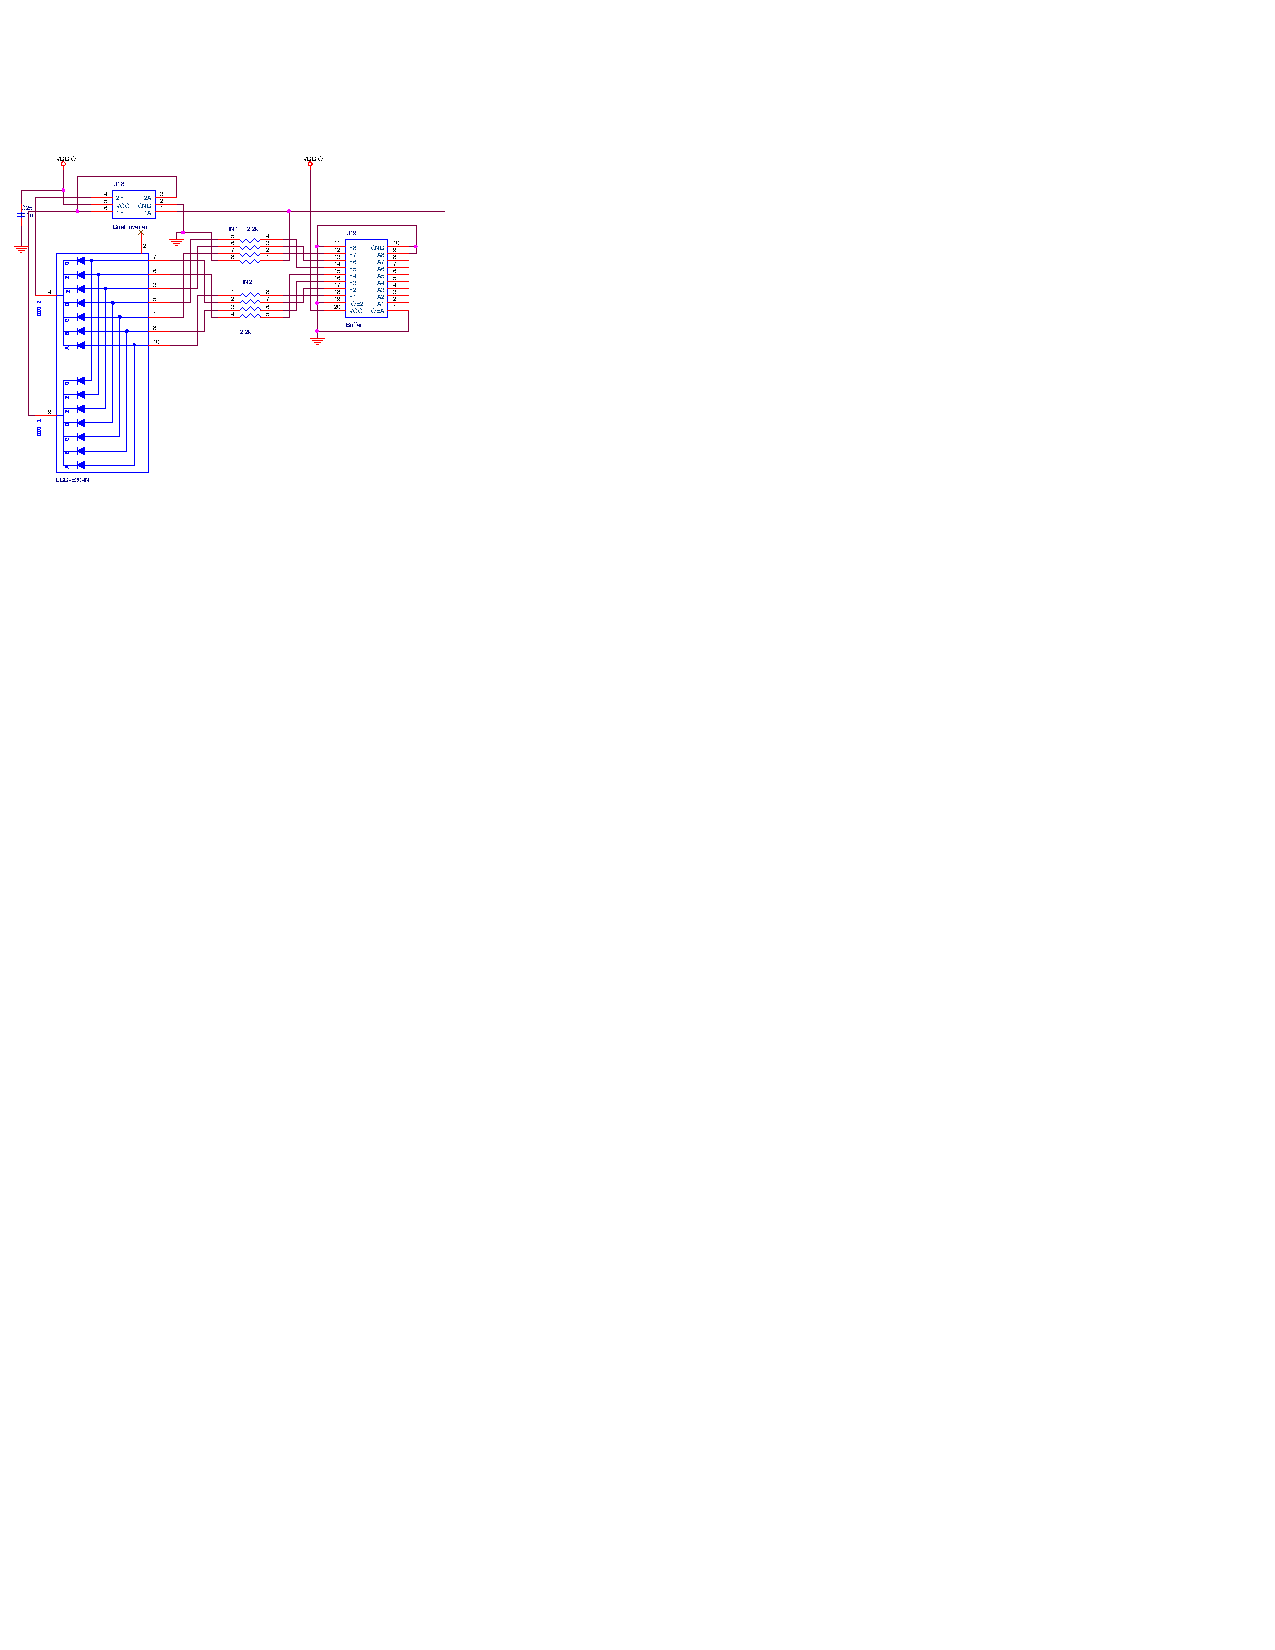
\includegraphics[scale=1.3]{Hardware/Figures/hardware-schematic_seven_segment.pdf}
		\caption{Prototyping Board Seven Segment Circuitry}
		\label{fig:hardware:schematic_seven_segment}
	\end{centering}
\end{figure}

The operation of the SPI in peer-to-peer mode is described in detail in Chapter \ref{sec:spi}, but it is important to mention that both nodes will be configured as slaves, which means that the associated pins will be floating. To prevent unpredictable behavior, pull-up and pull-down resistors are used on the SPICLK, SPISIMO, and SPISTE pins, as shown in Figure \ref{fig:hardware:schematic_links}. An LED is connected via a buffer to the MARB line so that it lights whenever a transfer is active on the link.

\begin{figure}[ptb]
	\begin{centering}
		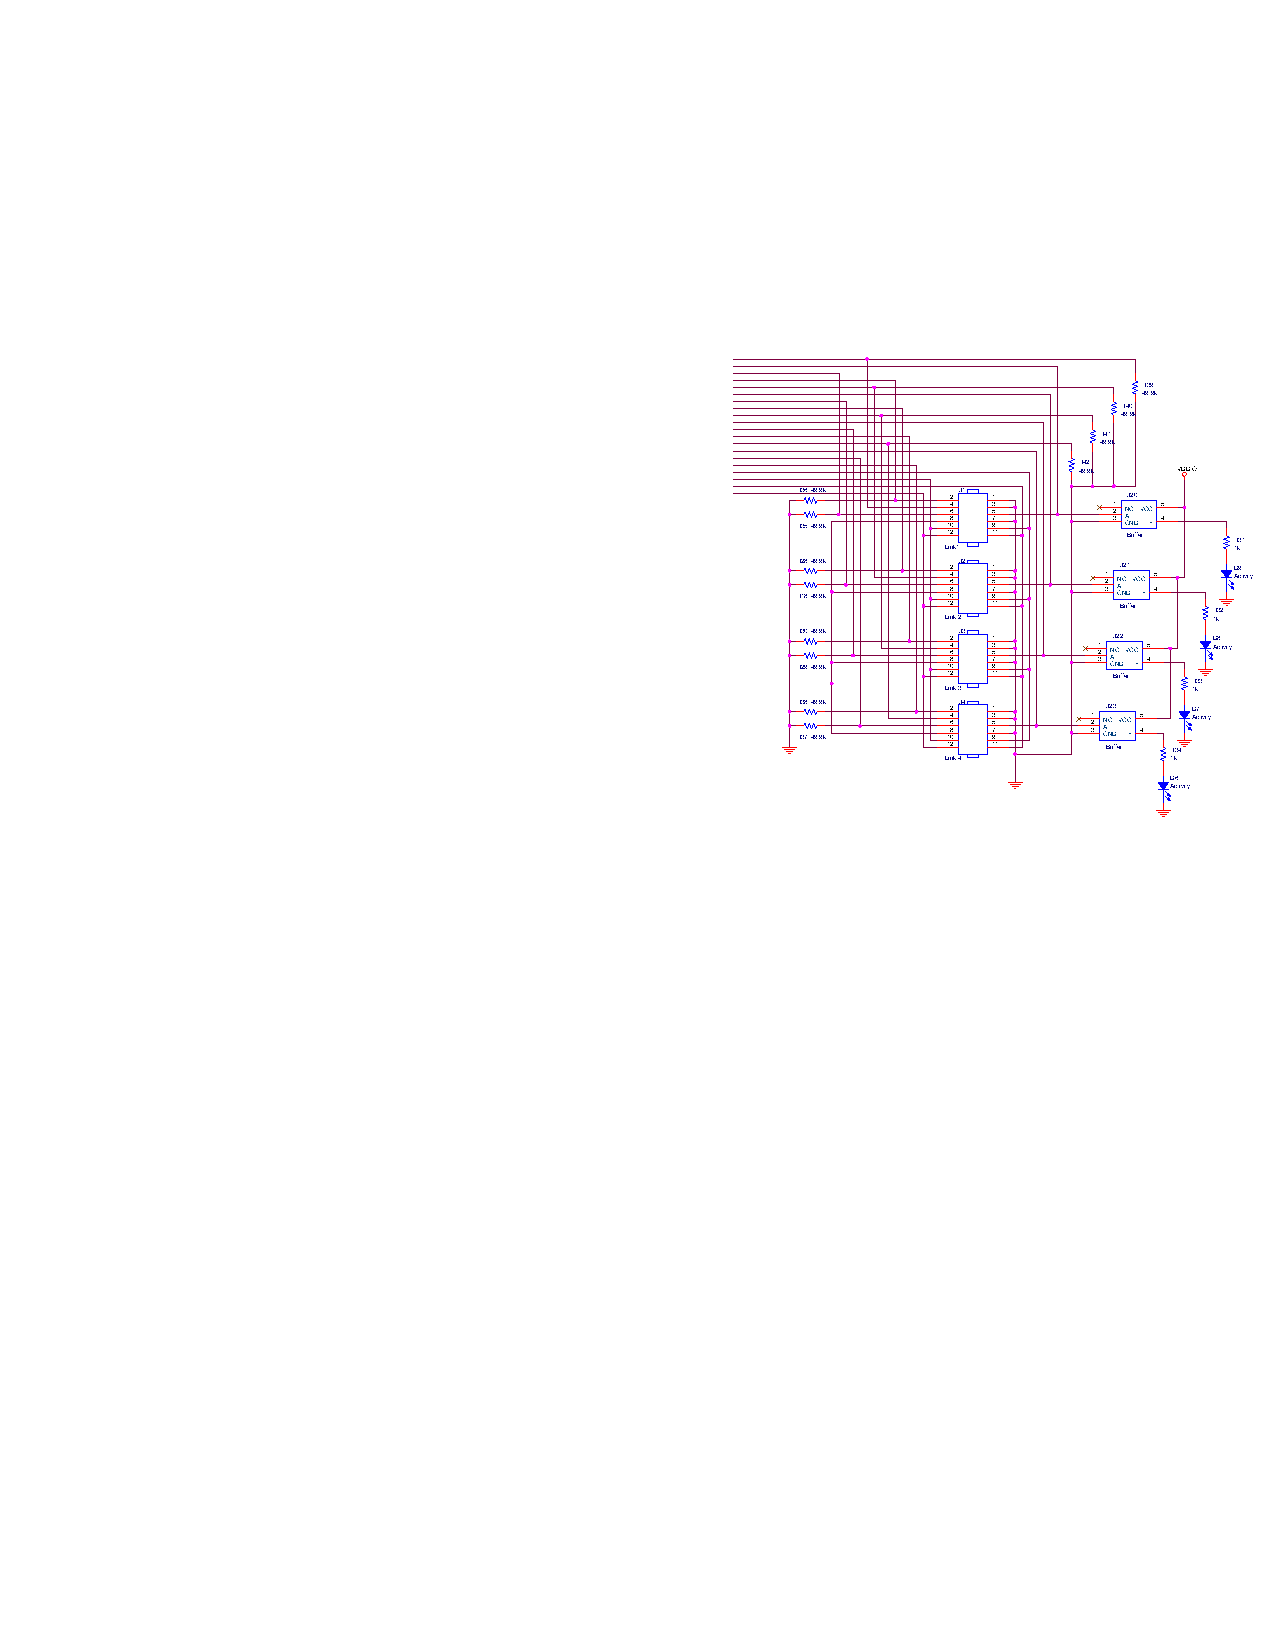
\includegraphics[scale=1.3]{Hardware/Figures/hardware-schematic_links.pdf}
		\caption{Prototyping Board Link Circuitry}
		\label{fig:hardware:schematic_links}
	\end{centering}
\end{figure}

\section{Results}\label{sec:hardware:results}

The boards were developed in an incremental fashion: a board was designed, and then three boards were manufactured based on the design\footnote{Ordering three boards is the sweet spot between price and quantity at Sierra Circuits, Inc.}. A total of nine boards were manufactured, with the last three boards based on the designs presented in Section \ref{sec:hardware:implementation}. One of the version 3 boards is shown running in Figure \ref{fig:hardware:board_running}. The best way to comprehensively test a board is to run software on it and so Figure \ref{fig:hardware:board_running} shows one of the boards running the final version of the firmware. The three horizontal lines next to the numeral 6 indicate that the firmware completed all operations, which wouldn't be possible if the boards didn't fully work. A few small modifications were made to the boards to get them fully functional: one of the pull-down resistors on the link was unnecessary and was removed, another pull-down resistor was changed to a pull-up resistor, and the enable signals between the seven segment display and the dual inverter were swapped to correct a design mistake using No. 30 AWG wire.
\begin{figure}[ptb]
	\begin{centering}
		\includegraphics[width=6in]{Hardware/Figures/hardware-board_running.png}
		\caption{Prototyping Board Running}
		\label{fig:hardware:board_running}
	\end{centering}
\end{figure}

\section{Future Work}\label{sec:hardware:future_work}

The boards are pretty complete, but a few odds and ends could use improvement. As mentioned earlier, the latest board revisions still had a few errors to be corrected. In the future, these changes should be incorporated into the board design itself instead of relying on post-production modifications. Chances to the link header, described in Chapter \ref{sec:spi}, will also require updates to the board design. Configuring the Analog to Digital Converter (ADC) on these boards with a header for connecting devices could be useful for future work on distributed I/O, as would setting up a header for connecting external devices directly to the extra GPIO pins in the link header that were not used. The testing process for the later chapters has revealed that a reset switch on each board would have also been useful.

\section{Conclusions}\label{sec:hardware:conclusions}

In this chapter, a network prototyping board was presented that allows rapid prototyping of different network topologies. Each prototyping board consists of an F2808 DSC, a JTAG connector, a Seven Segment Display, DIP switches for run-time configuration, four peer-to-peer SPI links, and onboard power circuitry for protection and regulation. The board has been tested and verified to be fully functional with the final firmware. 


